\documentclass[sigconf]{acmart}
\settopmatter{printacmref=false} % Removes citation information below abstract
\pagestyle{plain} % removes running headers
\renewcommand\footnotetextcopyrightpermission[1]{} % removes footnote with conference information in first column

\usepackage{booktabs} % For formal tables
\usepackage{adjustbox}
\usepackage{multirow}
\usepackage{amsmath}
\usepackage[linesnumbered,ruled]{algorithm2e}
%\usepackage{algorithm}% http://ctan.org/pkg/algorithm
%\usepackage{algpseudocode}% http://ctan.org/pkg/algorithmicx
% Copyright
%\setcopyright{none}
%\setcopyright{acmcopyright}
%\setcopyright{acmlicensed}
\setcopyright{rightsretained}
%\setcopyright{usgov}
%\setcopyright{usgovmixed}
%\setcopyright{cagov}
%\setcopyright{cagovmixed}


% DOI
%acmDOI{10.475/123_4}

% ISBN
%acmISBN{123-4567-24-567/08/06}

%Conference
%\acmConference[WOODSTOCK'97]{ACM Woodstock conference}{July 1997}{El
%  Paso, Texas USA}
%\acmYear{1997}
%\copyrightyear{2016}

%\acmPrice{15.00}

%\acmSubmissionID{123-A12-B3}

\begin{document}
\title{JointDNN: An Efficient Training and Inference Engine for Intelligent Mobile Cloud Computing Services}
%titlenote{Produces the permission block, and
% copyright information}
%subtitle{Extended Abstract}
%subtitlenote{The full version of the author's guide is available as
% \texttt{acmart.pdf} document}

% \textbf{HERE IS THE STORY: \\
% Here is a problem \\
% It's an interesting problem \\
% It's an unsolved problem \\
% Here is my idea \\
% My idea works (details, data) \\
% Here's how my idea compares to other people's approaches} \\

% \textbf{Saeed questions:} \\ 
% spelling: mobile-device or mobile device, make it consistent \\
% layer, filter, output of layer, channel \\
% Change GPU4DNN to a more recent reference \\
% Cite this maybe: [NIPS 2017] Towards Accurate Binary Convolutional Neural Network
% Yanzhi
% Single only platform, use the terminology the first time it has been used, check for dash! 

\author{Amir Erfan Eshratifar}
% \authornote{Dr.~Trovato insisted his name be first.}
% \orcid{1234-5678-9012}
\affiliation{
\department{Dept. of Electrical Engineering}
\institution{University of Southern California}
%\streetaddress{P.O. Box 1212}
\city{Los Angeles}
\state{California}
\postcode{43017-6221}
}
\email{eshratif@usc.edu}

\author{Mohammad Saeed Abrishami}
% \authornote{Dr.~Trovato insisted his name be first.}
% \orcid{1234-5678-9012}
\affiliation{
\department{Dept. of Electrical Engineering}
\institution{University of Southern California}
%\streetaddress{P.O. Box 1212}
\city{Los Angeles}
\state{California}
\postcode{43017-6221}
}
\email{abri442@usc.edu}

\author{Massoud Pedram}
% \authornote{Dr.~Trovato insisted his name be first.}
% \orcid{1234-5678-9012}
\affiliation{
\department{Dept. of Electrical Engineering}
\institution{University of Southern California}
%\streetaddress{P.O. Box 1212}
\city{Los Angeles}
\state{California}
\postcode{43017-6221}
}
\email{pedram@usc.edu}

% The default list of authors is too long for headers.
%renewcommand{\shortauthors}{B. Trovato et al.}


\begin{abstract}
Deep Neural Networks (DNNs) are among the most influential architectures of deep learning algorithms, being deployed in many mobile intelligent applications. End-side services, such as intelligent personal assistants (IPAs), autonomous cars, and smart home services often employ either simple local models or complex remote models on the cloud. Mobile-only and cloud-only computations are currently the status-quo approaches. In this paper, we propose an efficient, adaptive, and practical engine, JointDNN, for collaborative computation between a mobile device and cloud for DNNs in both inference and training phase. JointDNN not only provides an energy and performance efficient method of querying DNNs for the mobile side, but also benefits the cloud server by reducing the amount of its workload and communications compared to the cloud-only approach. Given the DNN architecture, we investigate the efficiency of processing some layers on the mobile device and some layers on the cloud server. We provide optimization formulations at layer granularity for forward and backward propagation in DNNs, which can adapt to mobile battery limitations and cloud server load constraints and quality of service. JointDNN achieves up to $18\times$ and $32\times$ reductions on the latency and mobile energy consumption of querying DNNs compared to the status-quo approaches, respectively.
\end{abstract}
\keywords{mobile cloud computing, deep learning, deep neural networks, intelligent services}


\maketitle

\section{Introduction}

% \textbf{STYLE: Describe the problem, State your contributions - introduction makes claims >> The body of the paper provides evidence to support each claim}
% \textbf{STYLE: Use references here}

%  Application:  unmanned drones, intelligent glasses

% Terminology:
% Filter layer: convolutional kernel
% Output of layer: activation

% In general, the computational complexity of CNNs is dominated by the convolutional layers, while the number of parameters is mainly related to the fully connected layers

% Why is sparsity important: The high sparsity of the parameters after pruning introduces two benefits for deep neural networks. On the one hand, the sparse parameters after pruning require less disk storage since the parameters can be stored in the compressed sparse row format (CSR) or compressed sparse column (CSC) format. On the other hand, computations involving those pruned parameters are omitted; thus, the computational complexity of deep networks can be reduced.

% According to the granularity of the pruning, pruning methods can be categorized into five groups: (Figure 2 in recent advances in efficient computation
% fine-grained pruning, 
% vector-level pruning, 
% kernel level pruning, 
% group-level pruning
% filter-level pruning

% Pruning helps better generalization and of course model will require less number of training samples, 

% 1. Fine-grained tuning: 
% Good reference for early pruning [NIPS 1989, Yann LeCun], [1993, Babak Hassibi] using approximate second-order derivatives of the loss function w.r.t. the parameters  to determine the saliency of the parameters

%% APPLICATIONS and their PAPERS:
% From Edge-Host [Georgia-DAC]: example is a camera network with edge devices composed of an image sensor and a lightweight processor.
% From Edge-Host [Georgia-DAC] applications: This configuration is appealing in the applications where the host make central decision and control
% Vehicle detection and recognition: Yong Tang et al. Vehicle detection and recognition for intelligent traffic surveillance system.
% Remote monitoring: G. Chen et al. Deep convolutional neural network based species recognition for wild animal monitoring
% Scene analysis: Cong Zhang et al. Cross-scene crowd counting via deep convolutional neural networks. In CVPR, 2015.

% From Zeiler paper: (i) the availability of much larger training sets, with millions of labeled examples; (ii) powerful GPU implementations, making the training of very large models practical and (iii) better model regularization strategies, such as Dropout.

% From BranchyNet: Due to the computational costs of deep networks, improving the efficiency of feedforward inference has been heavily studied. Two such approaches are network compression and implementation optimization. Network compression schemes aim to reduce the the total number of model parameters of a deep network and thus reduce the amount of computation required to perform inference.

% From XNOR-NET: virtual reality and augmented reality

DNN architectures are promising solutions in achieving remarkable results in a wide range of machine learning applications, including, but not limited to computer vision, speech recognition, language modeling and autonomous cars. 

Currently, there is a major growing trend in introducing more advanced DNN architectures and employing them in end-user applications. The considerable improvements in DNNs are usually achieved by increasing complexity which requires more computational resources for training and inference. Recent research directions to make this progress sustainable are: development of Graphical Processing Units (GPUs) as the vital hardware component of both servers and mobile devices~\cite{GPU4NN}, design of efficient algorithms for large-scale distributed training~\cite{DistributedDNN} and efficient inference~\cite{SAMRAGH}, compression and approximation of models~\cite{efficientDNN}, and most recently introducing collaborative computation of cloud and fog as known as dew computing~\cite{DewComputing}. 

Using cloud servers for computation and storage is becoming extensively favorable due to technical advancements and improved accessibility. Scalability, low cost, and satisfactory Quality of Service (QoS), made offloading to cloud the typical choice for computing intensive tasks. On the other side, mobile-device are being equipped with more powerful general purpose CPUs and GPUs. Very recently there is a new trend in hardware companies to design dedicated chips to better tackle machine-learning tasks. For example, Apple's A11 Bionic chip~\cite{iPhoneX} used in iPhone X uses a neural engine in its GPU to speed up DNN queries of applications such as face identification and facial motion capture~\cite{animoji}. 

There are currently two methods for DNN inference: mobile only and cloud only. In simple models, a mobile device is responsible for performing all of the computation. In case of complex models, the raw input data (image, video stream, voice, etc.) is uploaded and then computed on the cloud. The results of the task are later downloaded to the device. 

Besides the improvements of the mobiles devices mentioned earlier, the computational power of mobile devices are still considered significantly weaker than the cloud ones. Therefore, mobile-only approach can cause large inference latency and failure in meeting QoS. Moreover, embedded devices undergo major energy consumption constraints due to battery capacity limits. On the other hand, cloud-only suffers communication overhead for uploading the raw data and downloading the outputs. Moreover, slowdowns caused by service congestions, subscription costs, and network dependency should be considered as downsides of this approach. 

The superiority and persistent improvement of DNNs is heavily dependent on providing huge amount of training data. Typically, this data is collected from different resources and later fed into network for training. The final model can then be delivered to different devices for inference functions. However, there is a trend of appearance of applications requiring adaptive learning in online environments, such as self driving cars and security drones \cite{AdaptiveCar}\cite{EASI}. Model parameters in these smart devices are constantly being changed based on their continuous interaction with surroundings. Complexity of these architectures with extended number of parameters and current cloud-only methods for DNN training, implies a constant communication cost and burden of increased power consumption for mobile device. 

Automatic partitioning of computationally extensive tasks over the cloud for optimization of performance and energy consumption has been already well studied~\cite{CloneCloud}. Most recently, scalable distributed hierarchy structures between end-user device, edge, and cloud have been suggested~\cite{CloudEdgeDevice} which are specialized for DNN applications. However, exploiting the layer granularity of DNN architectures for run time partitioning has not been studied throughly yet. 



\begin{figure}[h]
\centering
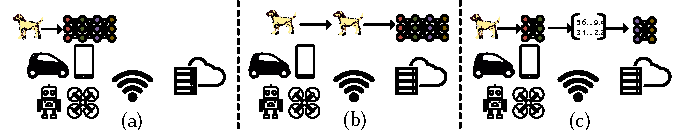
\includegraphics[width=\linewidth]{overall_system}
\caption{Different computation partitioning methods. (a) Mobile only: computation is completely done on mobile device. (b) Cloud only: raw input data is sent to cloud, computations is done on cloud and results are sent back to mobile device. (c) JointDNN: DNN architecture is partitioned at the granularity of layers, each layer can be computed either on cloud or mobile.}
\label{fig:fig_intro}
\end{figure}

% Story of the paper at the end of the introduction:
% Considering these char. we modeled it with a DAG
% Parameters of a DAG are
% Now you have a complete model, what do u want to solve, how do u want to solve it? Algorithm
% Parameters are extracted by experiments
% Results
% Conclusion
% Note: I did not mention the ILP for constraints! 
In this work, we are investigating inference and training of DNNs in a \textbf{joint} platform of mobile and cloud as an alternatives to the current single-platform methods as illustrated in Figure~\ref{fig:fig_intro}. Considering DNN architectures as an ordered sequence of layers, and possibility of computation of every layer either on mobile or cloud, we can model the DNN structure as a directed acyclic graph (DAG). The parameters of our real-time adaptive model are dependent on the following factors: mobile/cloud hardware and software resources, battery capacity, network specifications, and QoS. Based on this modeling, we show that the problem of finding the optimal computation schedule for different scenarios, i.e. best performance or energy consumption, can be reduced to the polynomial time shortest path problem. 

To present realistic results, we made experiments with real hardwares as mobile device and cloud. To model the communication between platform, we used different network technologies and the most recent reports on their specifications in the U.S. 

DNN architectures can be categorized based on functionality. These differences enforce specific type and order of layers in architecture, directly affecting the partitioning result in the collaborative method. For discriminative models, used in recognition applications, the layer size gradual decrease proceeding from input toward output~\ref{fig:DNN_category}. This sequence suggests computation of the first few layers on the mobile device to avoid excessive communication cost of uploading large raw input data. On the other hand, growth of the layer size from input to output in generative models used for synthesizing new data, implies the possibility of uploading small input to the cloud and later downloading and computing the last layers on the mobile device for better efficiency. Interesting mobile applications like image to image translation are implemented with autoencoder architectures, usually consisting of middle layers with smaller sizes compared to input and output. Consequently we expect the first and last layers to be computed on the mobile device in our collaborative approach. We examined eight well-known DNN benchmarks selected from these categories to illustrate their differences in collaborative computation approach. 

As we will see in Section~\ref{Results}, the communication between the mobile and cloud is the main bottleneck for both performance and energy in the collaborative approach. We investigated the specific characteristics of CNN layer outputs and introduced a lossless compression method to reduce the communication costs. 

State-of-the-art work for collaborative computation of DNNs~\cite{Neurosurgeon} only considers one offloading point, assigning computation of its previous layers and next layers on the mobile and cloud platforms, respectively. We show that this approach is non-generic and fails to be optimal, and introduced a new method granting the possibility of computation on either platforms for each layer independent of other layers. Our evaluations show that JointDNN significantly improves the latency and energy up to $3\times$ and $7\times$ respectively compared to the status-quo single platform approaches without any compression. The main contributions of this paper can be listed as:

\begin{itemize}
\item Introducing a novel model for collaborative computation between the mobile and cloud 
\item Formulating the problem of optimal computation scheduling of DNNs at layer granularity in mobile cloud computing environment as shortest path problem and integer linear programming (ILP) 
\item Examining compressibility of DNN layers and developing a lossless compression method to improve communication costs
\item Demonstrating the significant improvements of performance, mobile energy consumption, and cloud workload achieved by using \textbf{JointDNN}
\end{itemize}

\begin{figure}
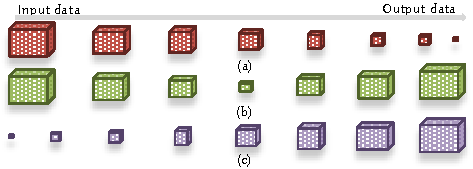
\includegraphics{architectures_layer_size}
\caption{Typical layer size architecture of (a) Discriminative (b) Autoencoder (c) Generative models.}
\label{fig:DNN_category}
\end{figure}


\section{Problem definition and modeling}
In this section, we explain the general architecture of DNN layers and our profiling method. Moreover, we elaborate on how the cost optimization can be reduced to a shortest path problem by introducing the JointDNN graph model. Finally, we show how the constrained problem is formulated by setting up ILP. 

\subsection{DNN Building Blocks}
DNNs are networks composed of several layers stacked to each other. We briefly explain the functionality of each layers used in the state-of-the-art architectures: 

\textbf{Convolution Layer} \textit{(conv)} consists of a set of filters with dimensions relatively smaller than their input. Each filter completely traverses through the input with a predefined step size and computes the dot product between it's parameters and the corresponding part of the input. This process creates different feature maps (referred to as channels) for different filters from the same input data. This aspect of preserving the locality of input features has made Convolutional Neural Network (CNN) architectures the horse power of the state-of-the-art image classification models. Because of dot product basis of \textit{conv}, it can be formulated as General Matrix Multiplication (GEMM), therefore capable of gaining performance improvement by using parallel computing devices (e.g. GPUs). 

\textbf{Fully Connected Layer} \textit{(fc)} is the main component of most regular neural networks in which every neuron is connected to all neurons of the previous layer. This fully pairwise connection architecture comprises large portion of computation of the whole network. Like \textit{conv}, \textit{fc} layer is also formulated as GEMM. 

% TODO: Major task of pooling: increasing the receptive field
\textbf{Pooling Layer} \textit{(pool)} performs a non-linear down sampling function over non-overlapping spatially local parts of input. Max-pooling is the most common function used in this type of layer alongside other functions such as average or L2-norm pooling. 

\textbf{Activation Layer} increases the non-linearity property of neural network architectures. This layer applies non-linear activation function on single data points of input to generate an output with the same size. Among various non-linear functions, such as sigmoid and hyperbolic tangent, Rectified Linear Unit \textit{(relu)} is currently the favorable choice in DNN architectures as it is simple and speeds up the tedious training process~\cite{ReLUpaper}. 

\textbf{Local Response Normalization} \textit{(lrn)} performs local normalization by imposing a local competition for big activities between adjacent features in a channel, and also between features at the same spatial location in different channels. \textit{lrn} are inspired by inhibition schemes observed in the brain helps with intention of generalization. There are different formulations suggested for \textit{lrn}, as shown in~\cite{AlexNet, multiStageArc} they may lead to slight improvements. 

% TODO: Consider p as probability of keeping the neuron active in training. During testing all neurons are present but their outputs are multiplied by p to maintain the scale of inputs. Add this to paper! 
\textbf{Dropout Layer} \textit{(drop)} 
As mentioned earlier, \textit{fc} occupies most of the parameters of DNN models and thus vulnerable to overfitting. Typically regularization methods are used to prevent overfitting by reducing high dependency of network on individual neurons during training. In dropout~\cite{DropOut} technique, at each training iteration every neurons can be removed (droped out) from network with a predetermined probability $p$ or kept with probability $1-p$ and the training is done on the remaining network. The dropped out nodes will have their previous weight for the next training iteration. 

\textbf{Deconvolution Layer} \textit{(deconv)} also known as transposed convolution is mostly used on generative and autoencoder models in applications such as building high-resolutions picture from low-resolution pictures and high-level descriptions. The goal in deconvolution is to find $f$ in the convolution equation of form $f*g=h$. In case of DNNs, $g$ is the filter and $f$ is the input of the convolution~\cite{Deconv}.

\textbf{Long Short-Term Memory Layer} \textit{(lstm)} is a building unit for layers of a recurrent neural network (RNN) and is widely used due to its promising results in speech recognition applications. A typical LSTM unit is composed of a cell, an input gate, an output gate and a forget gate, which is responsible for remembering and forgetting specific values over arbitrary time intervals. The whole LSTM unit can be thought as a typical artificial neuron, as in a feed-forward neural network.

\textbf{Softmax} \textit{(soft)} is the last layer in multi-class architectures, usually connected in a one-to-one correspondence way to a \textit{fc} layer. Softmax establishes a probability distribution by representing each class probability with a single neuron. 

% \begin{itemize}
% \item basic idea explained again: each node can be calculated either in mobile or cloud. Computation time on mobile, computation time on server, energy(power), P mobile, P cloud and comm. time.
% \item consecutive layers, explained in details in \textbf{ref 2 Experiments}. 
% \item The time of the communication is related to 1. amount of the data at the output of the layer \textbf{ref 2 Compression},  communication specifications \textbf{ref to communication spec}. 

% \item graph representation of the problem
% \item modeling of inference into graph
% \item modeling of training into graph
% \item reducing the problem to the shortest path problem, explaining the shortest path problem (complexity, etc. maybe here, implementation of the algorithm in results section)
% \item we will explain each DNN structure later \textbf{ref to different DNN structures} but here we should note that modeling the graph in some DNN (resNet) is more complicated and explained later. 
% \item What about constraints? They make this problem NP, \textbf{TODO:} possibly using ILP.

% \end{itemize}

\subsection{Energy and Latency Profiling}
\label{energy_latency_profiling}
There are three methods in measuring the latency and energy consumption of each layer in neural networks: 

\textbf{Statistical Modeling:} In this method, a regression model over the configurable parameters of operators (e.g. filter size in convolution) can be used to estimate the associated latency and energy. This method is prone to large error because of the inter-layer optimizations performed by DNN software packages. Therefore, it is necessary to consider execution of several consecutive operators grouped with each other during profiling. Many of these software packages are proprietary, making access to inter-layer optimization techniques impossible. 

% NVIDIA\textsuperscript{\textregistered} 

In order to illustrate this issue, we designed two experiments with 25 consecutive convolutions on NVIDIA Pascal\textsuperscript{\texttrademark} GPU using cuDNN\textsuperscript{\textregistered} library~\cite{cuDNN}. In the first experiment, we measure the latency of each convolution operator separately and set the total latency as sum of them. In the second experiment, we group the convolutions together and measure the total latency. All parameters are located on GPU's memory in both experiments, avoiding any data transfer from the main memory to make sure results are exactly representing the actual computation latency. 

% ALLIGN!

As we see in Figure~\ref{grouped_execution}, there is a large error gap between separated and grouped execution experiments which grows as the number of convolutions is increased. This observation confirms that we need to profile grouped operators to have more accurate estimations. Considering various consecutive combination of operators and different input sizes, this method requires a very large number of measurements, not to mention the need for a complex regression model.

% TODO: Erfan: Change it to layer count! Change the explanation! 
\begin{figure}
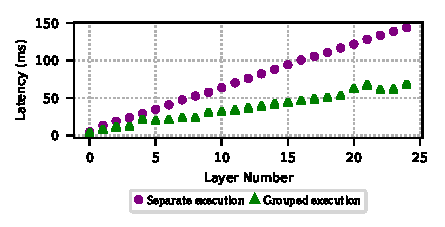
\includegraphics{consec}
\caption{Latency of grouped and separated execution of convolution operator.}\label{grouped_execution}
\end{figure}

\textbf{Analytical Modeling:} To derive an analytical approach for estimation of the latency and energy consumption, it is required to obtain the exact hardware and software specifications. However, the state-of-the-art work in latency modeling of DNNs~\cite{Paleo} fails to estimate layer-level delay within an acceptable error bound, for instance, underestimating the latency of a fully connected layer with 4096 neurons by around 900\%. Industrial developers do not reveal the detailed hardware architecture specifications and the proprietary parallel computing architectures such as CUDA\textsuperscript{\textregistered}, therefore, analytical approach could be quite challenging~\cite{GPUMODEL}.

\textbf{Application-specific Profiling:} In this method, the DNN architecture of the application being used is profiled in run-time. The number of applications in a mobile device using neural networks are generally limited. In conclusion, this method is more feasible, promising higher accuracy estimations. We have chosen this method for estimation of energies and latencies in the experiments of this paper. % HERE!

\subsection{JointDNN Graph Model}
First, we assume that a DNN is presented by a sequence of distinct layers with a linear topology as depicted in Figure~\ref{linear_topology}. Layers are executed sequentially, with output data generated by one layer feeds into the input of the next one. We denote the input and output data sizes of k$^{th}$ layer as $\alpha_k$ and $\beta_k$, respectively. Denoting the latency (energy) of layer k as $\omega_k$, where $k = 1, 2, ..., n$, the total latency (energy) of querying the DNN is $\sum_{k=1}^{n}{\omega_k}$.

% k$^{th}$

The mobile cloud computing optimal scheduling problem can be reduced to a shortest path problem, from node $S$ to $F$, in the graph of Figure~\ref{linear_topology_mc}. \textbf{Mobile Execution} cost of the k$^{th}$ layer ($C(ME_k)$) is the cost of executing the k$^{th}$ layer in the mobile while the cloud server is idle. \textbf{Cloud Execution} cost of the k$^{th}$ layer ($C(CE_k)$) is the executing cost of the k$^{th}$ layer in the cloud server while the mobile is idle. \textbf{Uploading the Input Data} cost of the k$^{th}$ layer is the cost of uploading output data of the (k-1)$^{th}$ layer to the cloud server $(UID_k)$. \textbf{Downloading the Input Data} cost of the k$^{th}$ layer is the cost of downloading output data of the (k-1)$^{th}$ layer to the mobile $(DID_k)$. The costs can refer to either latency or energy. However, as we showed in Section~\ref{energy_latency_profiling}, the assumption of linear topology in DNNs is not true and we need to consider all the consecutive grouping of the layers in the network. This fact suggests replacement of linear topology by a tournament graph as depicted in Figure~\ref{packing_topology}. We define the parameters of this new graph, \textit{JointDNN graph model}, in Table~\ref{jointDNNGraphParam}. 

\begin{figure}[t]
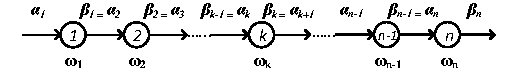
\includegraphics{linear_topology}
\caption{Computation model in linear topology.}\label{linear_topology}
\end{figure}

\begin{figure}[t]
%\includegraphics[height=1in, width=1in]{fly}
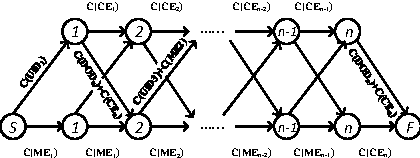
\includegraphics{linear_topology_mc}
\caption{Graph representation of mobile cloud computing optimal scheduling problem for linear topology.}
\label{linear_topology_mc}
\end{figure}


\begin{table}[b]
\caption{Parameter Definition of Graph Model} % title of Table
\label{nonlin_inputs} % is used to refer this table in the text
\centering % used for centering table
\begin{tabular}{|c|c|} % centered columns (4 columns)
\hline %inserts double horizontal lines
\textbf{Param.} & \textbf{Description of Cost}\\ [0.5ex] % inserts table
%heading
\hline % inserts single horizontal line
$CE_{i:j}$ & Executing layers $i$ to $j$ on the cloud \\
\hline % inserts single horizontal line
$ME_{i:j}$ & Executing layers $i$ to $j$ on the mobile \\
\hline % inserts single horizontal line
$ED_{i,j}$ & $CE_{i:j}$ + $DID_j$\\
\hline % inserts single horizontal line
$EU_{i,j}$ & $ME_{i:j}$ + $UID_j$\\
\hline % inserts single horizontal line
$\phi_{k}$ & All the following edges: $\forall i=1:k-1$ $ED_{i,k-1}$\\
\hline % inserts single horizontal line
$\Omega_{k}$ & All the following edges: $\forall i=1:k-1$ $ME_{i,k-1}$\\
\hline % inserts single horizontal line
$\Psi_{k}$ & All the following edges: $\forall i=1:k-1$ $EU_{i,k-1}$\\
\hline % inserts single horizontal line
$\Gamma_{k}$ &  All the following edges: $\forall i=1:k-1$ $CE_{i,k-1}$\\
\hline % inserts single horizontal line
$\Pi_m$ & All the following edges: $\forall i=1:n$ $ME_{i,n}$\\
\hline % inserts single horizontal line
$\Pi_c$ & All the following edges: $\forall i=1:n$ $ED_{i,n}$\\
\hline % inserts single horizontal line
$U_1$ & Uploading the input of the first layer\\
\hline %inserts single line
\end{tabular}
\label{jointDNNGraphParam}
\end{table}

\begin{figure*}
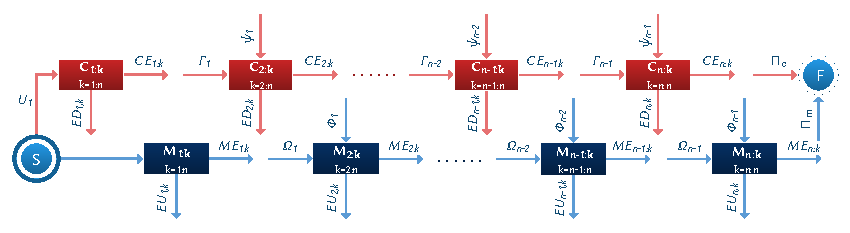
\includegraphics{packing_topology}
\caption{JointDNN graph model.}
\label{packing_topology}
\end{figure*}

% We introduce two dummy nodes: node S as the starting node and node F as the finishing node. 

% the k$^{th}$ layer

In this graph, node $C_{i:j}$ represents that the layers $i$ to $j$ are computed on the cloud server, while node $M_{i:j}$ represents that the layers $i$ to $j$ are computed on the mobile device. An edge between two adjacent nodes in JointDNN graph model is associated with four possible cases: 1) A transition from the mobile to the mobile, which only includes the mobile computation cost ($ME_{i,j}$) 2) A transition from the cloud to the cloud, which only includes the cloud computation cost ($CE_{i,j}$) 3) A transition from the mobile to the cloud, which includes the mobile computation cost and uploading cost of the inputs of the next node ($EU_{i,j} = ME_{i,j} + UID_{j+1}$) 4) A transition from the cloud to the mobile, which includes the cloud computation cost and downloading cost of the inputs of the next node ($ED_{i,j} = CE_{i,j} + DID_{j+1}$). Under this formulation, we can transform the computation scheduling problem to finding the shortest path from $S$ to $F$. 

Residual networks are a class of powerful and easy-to-train architectures of DNNs~\cite{ResNet}. 


In residual networks, as depicted in Figure~\ref{resnet} (a), the output of one layer is fed into another layer with distance of at least two. Thus, we need to keep track of the source layer (node $2$ in Figure~\ref{resnet}) so as to know that this layer is computed on the mobile or the cloud. 

Our standard graph model has a memory of one which is the very previous layer. We provide a method to transform the computation graph of this type of network to our standard model, JointDNN graph. 

In this regard, we add two additional chains of size $k-1$, where $k$ is the number of nodes in the residual block ($3$ in Figure~\ref{resnet}). One chain represents the case of computing layer $2$ on the mobile and the other one represents the case of computing layer $2$ on the cloud. In Figure~\ref{resnet}, we have only shown the weights that need to be modified, where $D_2$ and $U_2$ are the cost of downloading and uploading the output of layer $2$, respectively.

By solving the shortest path problem in JointDNN graph model, we can obtain the optimal scheduling of inference in DNNs. Online training consists of one inference and one back-propagation step. The total number of layers is noted by $N$ consistently throughout this paper so there are $2N$ layers for modeling training, where the second $N$ layers are the mirrored version of the first $N$ layers, and their associated operations are the gradients of the error function with respect to the DNN's weights. The main difference between the mobile cloud computing graph of inference and online training is the need for updating the model by downloading the new weights from the cloud. We assume that the cloud server performs the whole back-propagation step separately, even if it is scheduled to be done on the mobile, therefore, there is no need for mobile device to upload the weights that are updated by itself in order to save mobile energy consumption. The modification in JointDNN graph model is adding the costs of downloading weights of the layers that are updated in the cloud to $ED_{i,j}$.

The shortest path problem can be solved in polynomial time efficiently. 

However, the problem of shortest path subjected to constraints has been shown to be NP-Complete~\cite{NPComplete}. For instance, assuming our standard graph is constructed for energy and we need to find the shortest path subject to the constraint of the total latency of that path being less than a time deadline (QoS). However, there is an approximation solution to this problem, "LARAC" algorithm~\cite{LARAC}, the nature of our application does not require to solve this optimization problem frequently, therefore, we aim to obtain the optimal solution. We can constitute a small look-up table of optimization results for different set of parameters (e.g. network bandwidth, cloud server load, etc.). We provide the ILP formulations of DNN partitioning in the following sections.

\begin{figure}[b]
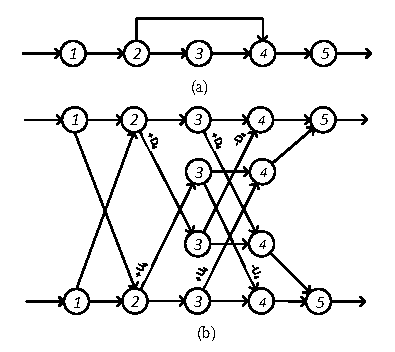
\includegraphics{resnet}
\caption{(a) A residual building block (b) Transformation of a residual building block into shortest path problem.}\label{resnet}
\end{figure}

\subsection{ILP Setup}

\subsubsection{Performance Efficient Computation Offloading ILP Setup for Inference}

We formulated the scheduling of inference in DNNs as an ILP with tractable number of variables. In our method, first we profile the delay and energy consumption of consecutive layers of size $m$ $\in$ $\{1, 2,\dots, N\}$. Thus, we will have
  \begin{equation}
      \begin{split}
N + (N-1) + ... + 1 = N(N+1)/2
  \end{split}
\end{equation}
number of different profiling values for delay and energy.
Considering layer $i$ to layer $j$ to be computed either on the mobile device or cloud server, we assign two binary variables $m_{i,j}$ and $c_{i,j}$, respectively. Download and upload communication delays needs to be added to the execution time, when switching from/to cloud to/from mobile, respectively.

\begin{equation}
      \begin{split}
T_{computation} &= \sum_{i=1}^{n}{\sum_{j=i}^{n}{
(m_{i,j}.T_{mobile_{L_{i,j}}} + c_{i,j}.T_{cloud_{L_{i,j}}})
}}
  \end{split}
\end{equation}
  \begin{equation}
      \begin{split}
T_{communication} &= \sum_{i=1}^{n}{\sum_{j=i}^{n}{\sum_{k=j+1}^{n}{m_{i,j}.c_{j+1,k}.T_{upload_{L_j}}}}} \\
& + \sum_{i=1}^{n}{\sum_{j=i}^{n}{\sum_{k=j+1}^{n}{c_{i,j}.m_{j+1,k}.T_{download_{L_j}}}}} \\
& + \sum_{i=1}^{n}{c_{1,i}.T_{upload_{L_i}}} \\
& + \sum_{i=1}^{n}{c_{i,n}.T_{download_{L_n}}}
  \end{split}
  \label{eq: full_pass_comm}
\end{equation}

\begin{equation}
T_{total} = T_{computation} + T_{communication}\thinspace\thinspace\thinspace\thinspace\thinspace\thinspace\thinspace\thinspace\thinspace\thinspace\thinspace\thinspace\thinspace\thinspace\thinspace\thinspace\thinspace\thinspace\thinspace\thinspace\thinspace\thinspace\thinspace\thinspace\thinspace\thinspace\thinspace\thinspace\thinspace\thinspace\thinspace
\end{equation}

$T_{mobile_{L_{i,j}}}$ and $T_{cloud_{L_{i,j}}}$ represent the execution time of the i$^{th}$ layer to the j$^{th}$ layer on the mobile and cloud, respectively. $T_{download_{L_i}}$ and $T_{upload_{L_i}}$ represent the latency of downloading and uploading the output of the i$^{th}$ layer, respectively. Considering each set of the consecutive layers, whenever $m_{i,j}$ and one of $\{c_{j+1,k}\}_{k=j+1:n}$ are equal to one, the output of the j$^{th}$ layer is uploaded to the cloud. The same argument applies to downloading.
We also note that the last two terms in Eq.~\ref{eq: full_pass_comm} represent the condition by which the last layer is computed on the cloud and we need to download the output to the mobile device, and the first layer is computed on the cloud and we need to upload the input to the cloud, respectively. To support for residual architectures, we need to add a pair of download and upload terms similar to the first two terms in Eq.~\ref{eq: full_pass_comm} for the starting and ending layers of each residual block. In order to guarantee that all layers are computed exactly once, we need to add the following set of constraints:

\begin{equation}
	\begin{split}
		\forall m \in {1:n}: \sum_{i=1}^{m}{\sum_{j=m}^{n}{(m_{i,j} + c_{i,j})}} = 1
  	\end{split}
\end{equation}

Because of the non-linearity of multiplication, an additional step is needed to transform Eq.~\ref{eq: full_pass_comm} to the standard form of ILP. We define two sets of new variables:

\begin{equation}
\label{eq: download_upload_binary_var} 
	\begin{aligned}
      &u_{i,j} = m_{i,j}.\sum_{k=j+1}^{n}{c_{j+1,k}} \\
      &d_{i,j} = c_{i,j}.\sum_{k=j+1}^{n}{m_{j+1,k}}
     \end{aligned}
\end{equation}

with the following constraints:

\begin{equation}\label{eq: download_upload_constraints} 
	\begin{aligned}
      &u_{i,j} \leq m_{i,j}\\
      &u_{i,j} \leq \sum_{k=j+1}^{n}{c_{j+1,k}} \\
      &m_{i,j} + \sum_{k=j+1}^{n}{c_{j+1,k}} - u_{i,j} \leq 1\\
      &d_{i,j} \leq c_{i,j}\\
      &d_{i,j} \leq \sum_{k=j+1}^{n}{m_{j+1,k}} \\
      &c_{i,j} + \sum_{k=j+1}^{n}{m_{j+1,k}} - d_{i,j} \leq 1
	\end{aligned}
\end{equation}

The first two constraints ensure that $u_{i,j}$ will be zero if either $m_{i,j}$ or $\sum_{l=j+1}^{n}{c_{j+1,l}}$ are zero. The third inequality guarantees that $u_{i,j}$ will take value one if both binary variables, $m_{i,j}$ and $\sum_{l=j+1}^{n}{c_{j+1,l}}$, are set to one. The same reasoning works for $d_{i,j}$. In summary, the total number of variables in our ILP formulation will be $4N(N+1)/2$, where $N$ is total number of layers in the network. 

\subsubsection{Energy Efficient Computation Offloading ILP Setup for Inference}
Because of the nature of the application, we only care about the energy consumption on the mobile side. We formulate ILP as follows:
  \begin{equation}
      \begin{split}
E_{computation} &= \sum_{i=1}^{n}{\sum_{j=i}^{n}{
m_{i,j}.E_{mobile_{L_{i,j}}}}\thinspace\thinspace\thinspace\thinspace\thinspace\thinspace\thinspace\thinspace\thinspace\thinspace\thinspace\thinspace\thinspace\thinspace\thinspace\thinspace\thinspace\thinspace\thinspace\thinspace\thinspace\thinspace\thinspace\thinspace\thinspace\thinspace\thinspace\thinspace\thinspace\thinspace\thinspace\thinspace\thinspace\thinspace\thinspace\thinspace}\label{eq: energy_comp}
  \end{split}
\end{equation}
  \begin{equation}
      \begin{split}
E_{communication} &= \sum_{i=2}^{n}{\sum_{j=i}^{n}{m_{i,j}.E_{download_{L_i}}}} \\
& + \sum_{i=1}^{n}{\sum_{j=i}^{n-1}{m_{i,j}.E_{upload_{L_j}}}} \\
& + (\sum_{i=1}^{n}{(1-m_{1,i}) - (n-1)).E_{upload_{L_1}}} \\
& + (\sum_{i=1}^{n}{(1-m_{i,n}) - (n-1)).E_{download_{L_n}}}\label{eq: energy_comm}
  \end{split}
\end{equation}
  \begin{equation}
E_{total} = E_{computation} + E_{communication}\thinspace\thinspace\thinspace\thinspace\thinspace\thinspace\thinspace\thinspace\thinspace\thinspace\thinspace\thinspace\thinspace\thinspace\thinspace\thinspace\thinspace\thinspace\thinspace
\end{equation}

$E_{mobile_{L_{i,j}}}$ and $E_{cloud_{L_{i,j}}}$ represent the amount of energy required to compute the i$^{th}$ layer to the j$^{th}$ layer on the mobile and cloud, respectively. $E_{download_{L_i}}$ and $E_{upload_{L_i}}$ represent the energy required to download and upload the output of i$^{th}$ layer, respectively.
Similar to performance efficient ILP constraints, each layer should be executed exactly once:

\begin{equation}
      \begin{split}
\forall m \in {1:n}: \sum_{i=1}^{m}{\sum_{j=m}^{n}{m_{i,j}}} \leq 1
  \end{split}
\end{equation}

The ILP problem can be solved for different set of parameters (e.g. different uplink and download speeds), and then the scheduling results can be stored as a look-up table in the mobile device. Moreover because the number of variables in this setup is tractable solving ILP is quick. For instance, solving ILP for AlexNet takes around 0.045 seconds on Intel(R) Core(TM) i7-3770 CPU with MATLAB\textregistered's intlinprog() function using primal simplex algorithm.\\
\subsubsection{Performance Efficient Computation Offloading ILP Setup for Training}
The ILP formulation of online training phase is very similar to that of inference. In online training we have $2N$ layers instead of $N$ obtained by mirroring the DNN, where the second $N$ layers are backward propagation. Moreover, we need to download the weights that are updated in the cloud to the mobile. We assume that the cloud server always has the most updated version of the weights and does not require the mobile device to upload the updated weights. The following terms need to be added for the ILP setup of training:

\begin{equation}
      \begin{split}
T_{computation} &= \sum_{i=1}^{2n}{\sum_{j=i}^{2n}{
(m_{i,j}.T_{mobile_{L_{i,j}}} + c_{i,j}.T_{cloud_{L_{i,j}}})
}}\label{eq: full_pass_comp}
  \end{split}
\end{equation}
  \begin{equation}
      \begin{split}
T_{communication} &= \sum_{i=1}^{2n}{\sum_{j=i}^{2n}{\sum_{k=j+1}^{2n}{m_{i,j}.c_{j+1,k}.T_{upload_{L_j}}}}} \\
& + \sum_{i=1}^{2n}{\sum_{j=i}^{2n}{\sum_{k=j+1}^{2n}{c_{i,j}.m_{j+1,k}.T_{download_{L_j}}}}} \\
& + \sum_{i=1}^{n}{c_{1,i}.T_{upload_{L_i}}} \\
& + \sum_{i=n+1}^{2n}{\sum_{j=i}^{2n}{c_{i,j}.T_{download_{W_{i}}}}}
  \end{split}
\end{equation}

\begin{equation}
T_{total} = T_{computation} + T_{communication}\thinspace\thinspace\thinspace\thinspace\thinspace\thinspace\thinspace\thinspace\thinspace\thinspace\thinspace\thinspace\thinspace\thinspace\thinspace\thinspace\thinspace\thinspace\thinspace\thinspace\thinspace\thinspace\thinspace\thinspace\thinspace\thinspace\thinspace\thinspace\thinspace\thinspace\thinspace
\end{equation}

\subsubsection{Energy Efficient Computation Offloading ILP Setup for Training}
  \begin{equation}
      \begin{split}
E_{computation} &= \sum_{i=1}^{2n}{\sum_{j=i}^{2n}{
m_{i,j}.E_{mobile_{L_{i,j}}}}\thinspace\thinspace\thinspace\thinspace\thinspace\thinspace\thinspace\thinspace\thinspace\thinspace\thinspace\thinspace\thinspace\thinspace\thinspace\thinspace\thinspace\thinspace\thinspace\thinspace\thinspace\thinspace\thinspace\thinspace\thinspace\thinspace\thinspace\thinspace\thinspace\thinspace\thinspace\thinspace\thinspace\thinspace\thinspace\thinspace}\label{eq: energy_comp_train}
  \end{split}
\end{equation}
  \begin{equation}
      \begin{split}
E_{communication} &= \sum_{i=2}^{2n}{\sum_{j=i}^{2n}{m_{i,j}.E_{download_{L_i}}}} \\
& + \sum_{i=1}^{2n}{\sum_{j=i}^{2n-1}{m_{i,j}.E_{upload_{L_j}}}} \\
& + (\sum_{i=1}^{2n}{(1-m_{1,i}) - (2n-1)).E_{upload_{L_1}}} \\
& + (\sum_{i=n+1}^{2n}\sum_{j=i}^{2n}{(1-m_{i,j}) - (n-1)}).E_{download_{W_{i}}}\label{eq: energy_comm_train}
  \end{split}
\end{equation}
  \begin{equation}
E_{total} = E_{computation} + E_{communication}\thinspace\thinspace\thinspace\thinspace\thinspace\thinspace\thinspace\thinspace\thinspace\thinspace\thinspace\thinspace\thinspace\thinspace\thinspace\thinspace\thinspace\thinspace\thinspace
\end{equation}

\subsubsection{Scenarios}
There can be different optimization scenarios defined for ILP as listed below:
\begin{itemize}
\item \textbf{Performance efficient computation:} In this case, it is sufficient to solve the ILP formulation for performance efficient computation offloading.
\item \textbf{Energy efficient computation:} In this case, it is sufficient to solve the ILP formulation for energy efficient computation offloading.
\item \textbf{Battery budget limitation:} In this case, based on the available battery, the operating system can decide to dedicate a specific amount of energy consumption to each application. By adding the following constraint to the performance efficient ILP formulation, our framework would adapt to battery limitations: 
\begin{equation}
\begin{split}
	E_{computation} + E_{communication} \leq E_{ubound}
\end{split}
\end{equation}

\item\textbf{Cloud limited resources:} In the presence of cloud server congestion or limitations on user's subscription, we can apply execution time constraints to each application to alleviate the server load:

\begin{equation}
\begin{split}
\sum_{i=1}^{n}{\sum_{j=i}^{n}{
c_{i,j}.T_{cloud_{L_{i,j}}}}} \leq T_{ubound}
\end{split}
\end{equation}

\item \textbf{QoS:} In this scenario, we minimize the required energy consumption while meeting a specified deadline:

\begin{equation}
      \begin{split}
min\{E_{computation} + E_{communication}\} \\
T_{computation} + T_{communication} \leq T_{QoS}
  \end{split}
\end{equation}


This constraint could be applied to both energy and performance efficient ILP formulations.
\end{itemize}

\begin{algorithm}
    \SetKwInOut{Input}{Input}
    \SetKwInOut{Output}{Output}

    \underline{function JointDNN} $(N,L_i,D_i,NB,NP)$\;
    \Input{
1: $N$: number of layers in the DNN\\
2: $L_i|i=1:N$: layers in the DNN\\
3: $D_i|i=1:N$: data size at each layer\\
4: $NB$: mobile network bandwidth\\
5: $NP$: mobile network uplink and downlink power consumption\\
}
    \Output{Optimal schedule of DNN}
  \For{$i = 0;\ i < N;\ i = i + 1$}{
  \For{$j = 0;\ j < N;\ j = j + 1$}{
    $Latency_{i,j}, Energy_{i,j}$ = ProfileGroupedLayers$(i,j)$\;
    }
  }
G,S,F = ConstructShortestPathGraph($N$,$L_i$,$D_i$,$NB$,$NP$) //S and F are start and finish nodes and G is the JointDNN graph model\\
    \eIf{no constraints}
      {
      	$schedule$ = \textbf{ShortestPath(G,S,F)}
      }
      {
      \If{Battery Limited Constraint} {
	$E_{comm} + E_{comp} \le E_{ubound}$ \\
      	$schedule$ = PerformanceEfficientILP($N$,$L_i$,$D_i$,$NB$,$NP$)
      }
            \If{Cloud Server Contraint} {
           $\sum_{i=1}^{n}{\sum_{j=i}^{n}{
c_{i,j}.T_{cloud_{L_{i,j}}}}} \leq T_{ubound}$\\
      	$schedule$ = PerformanceEfficientILP($N$,$L_i$,$D_i$,$NB$,$NP$)
      }
            \If{QoS} {
            $T_{comm} + T_{comp} \le T_{QoS}$ \\
      	$schedule$ = EnergyEfficientILP($N$,$L_i$,$D_i$,$NB$,$NP$)
      };\

      }
       return $schedule$\;
    \caption{JointDNN engine optimal scheduling of DNNs}
\end{algorithm}
\begin{figure*}
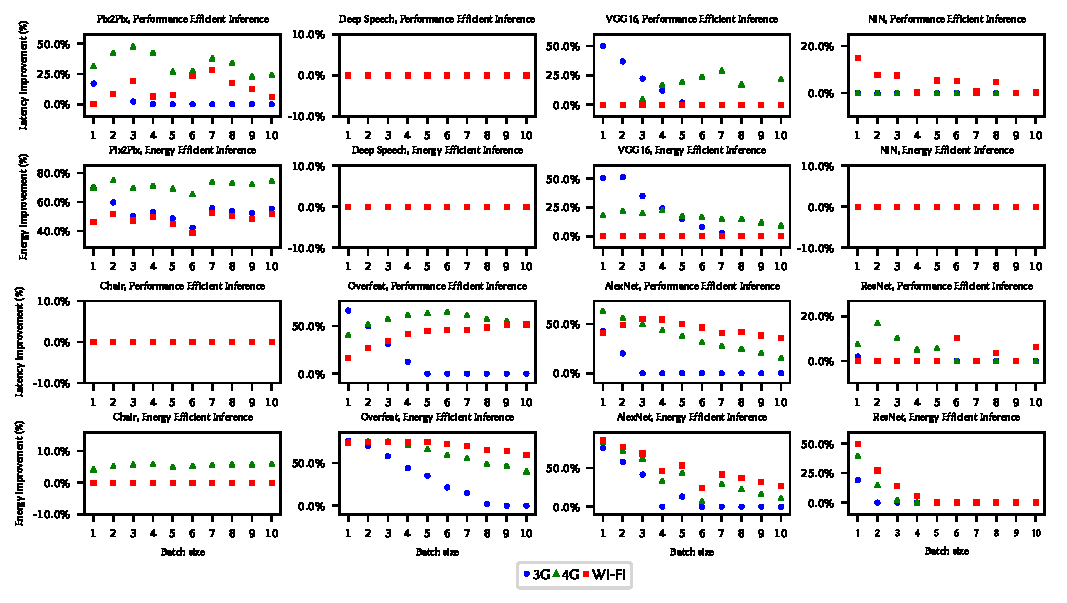
\includegraphics{inference_results}
\caption{Latency and energy improvements for different batch sizes during inference.}
\label{inference_results}
\end{figure*}

\begin{figure*}
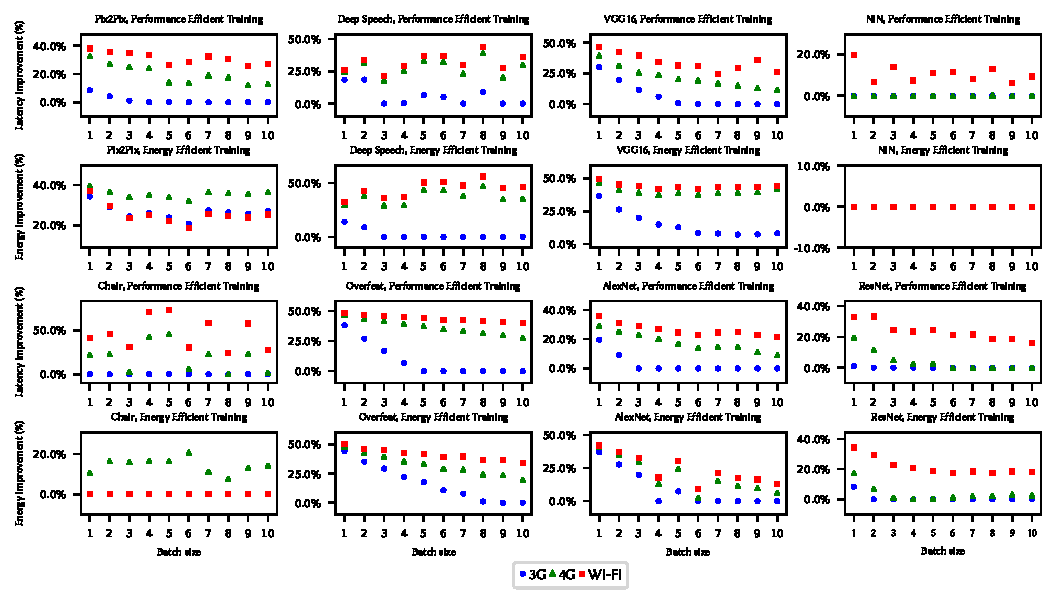
\includegraphics[width=\linewidth]{training_results}
\caption{Latency and energy improvements for different batch sizes during training.}
\label{training_results}
\end{figure*}

\section{Evaluation}

\subsection{Deep Architecture Benchmarks}

Since the architecture of neural networks depends on the type of the application, we have chosen three common application types of DNNs:

\begin{enumerate}
\item \textbf{Discriminative neural networks} are a class of models in machine learning for modeling the conditional probability distribution $P(y|x)$. This class generally is used in classification and regression tasks. AlexNet\cite{AlexNet}, OverFeat\cite{OverFeat}, VGG16\cite{VGG16}, Deep Speech\cite{DeepSpeech}, ResNet\cite{ResNet}, and NiN\cite{NiN} are well-known discriminative models we use as benchmarks in this experiment. Except Deep Speech, used for speech recognition, all other benchmarks are used in image classification tasks. 

\item \textbf{Generative neural networks} model the joint probability distribution $P(x,y)$, allowing generation of new samples. These networks have applications in Computer Vision~\cite{GAN} and Robotics~\cite{DeepVisual}, which can be deployed on a mobile device. Chair~\cite{Chair} is a generative model we use as benchmark in this work.
\item \textbf{Autoencoders} are another class of neural networks used to learn a representation for a data set. Their applications are image reconstruction, image to image translation, and denoising to name a few. Mobile robots can be equipped with autoencoders to be used in their computer vision tasks. We use Pix2Pix~\cite{Pix2Pix}, as a benchmark from this class.
\end{enumerate}

\begin{table}
\caption{Benchmark Specifications}
\centering
\begin{adjustbox}{center}
     %\begin{adjustbox}{center}
        \begin{tabular}{|c|c|c|}
        \hline
        \textbf Type & \textbf Model & \textbf Layers \\                
            \hline
            \multirow{4}{*}{Discriminative} & \multicolumn{1}{c}{AlexNet} & \multicolumn{1}{|c|}{21} \\\cline{2-3}
            & \multicolumn{1}{c}{OverFeat} & \multicolumn{1}{|c|}{14} \\\cline{2-3}
            & \multicolumn{1}{c}{Deep Speech} & \multicolumn{1}{|c|}{10} \\\cline{2-3}
            & \multicolumn{1}{c}{ResNet} & \multicolumn{1}{|c|}{70} \\\cline{2-3}
            & \multicolumn{1}{c}{VGG16} & \multicolumn{1}{|c|}{37} \\\cline{2-3}
            & \multicolumn{1}{c}{NiN} & \multicolumn{1}{|c|}{29} \\\hline
           Generative & Chair & 10 \\                \hline
            Autoencoder &  Pix2Pix & 32 \\                \hline
        \end{tabular}
     \end{adjustbox}
%     \vspace{ - 05 mm}

\label{benchmarks}
\end{table}

\begin{table}[h]
	\caption{Mobile networks specifications in the U.S.} 
	\centering 
	\begin{tabular}{|c|c|c|c|} \hline
	\textbf{Param.} & \textbf{3G} & \textbf{4G} & \textbf{Wi-Fi} \\ \hline
	Download speed (Mpbs)	& 	2.0275 	&	13.76 	&	54.97 \\ \hline
	Upload speed (Mbps)	&	1.1		&	5.85	&	18.88 \\ \hline
$\alpha_u$ (mW/Mpbs)	& 868.98	& 438.39	&	283.17    \\ \hline
$\alpha_d$ (mW/Mpbs)	 & 122.12 	& 51.97	&	137.01        \\ \hline
$\beta$ (mW)	& 817.88	& 1288.04	&	132.86            \\ \hline
\end{tabular}
\label{table:network_parameters} 
\end{table}

\subsection{Mobile and Server Setup}
We used Jetson TX2 module developed by NVIDIA\textsuperscript{\textregistered}~\cite{JetsonTX2}, a fair representative of mobile computation power as our mobile device. This module enables efficient implementation of DNN applications used in products such as robots, drones, and smart cameras. It is equipped with NVIDIA Pascal\textregistered GPU with 256 CUDA cores and a shared 8~GB 128~bit LPDDR4 memory between GPU and CPU. To measure the power consumption of the mobile platform, we used INA226 power sensor~\cite{INA226}. 

NVIDIA\textsuperscript{\textregistered} Tesla\textsuperscript{\textregistered} K40C~\cite{TeslaGPU} with 12~GB memory serves as our server GPU. The computation capability of this device is more than one order of magnitude compared to our mobile device. 
% TODO: Should I mention that we are not measuring the server power?
% TODO: Should we make the rows of the two tables the same? System? 
% TODO: textregistered sign in table 
% Reference on the table title?

\subsection{Communication Parameters}
To model the communication between platforms, we used the average download and upload speed of mobile Internet~\cite{MobNet, Speedtest} for different networks (3G, 4G and Wi-Fi) as shown in Table~\ref{table:network_parameters}.


The communication power for download ($P_d$) and upload ($P_u$) is dependent on the network throughput ($t_d$ and $t_u$). Comprehensive examinations in~\cite{4GLTE} indicates that uplink and downlink power can be modeled with linear equations (Eq.~\ref{eq:power_model_eq}) fairly accurate with less than 6\% error rate. Table~\ref{table:network_parameters} shows the parameter values of this equation for different networks. 

\begin{equation}
\begin{split}
P_u = \alpha_u t_u + \beta \\
P_d = \alpha_d t_d + \beta \label{eq:power_model_eq}
  \end{split}
\end{equation}



\section{Results}

The latency and energy improvements of inference and online training with our engine for 8 different benchmarks are shown in Figures~\ref{inference_results} and~\ref{training_results},  respectively. We considered the best case of mobile-only and cloud-only as our baseline. JointDNN can achieve up to 66\% and 86\% improvements in latency and energy consumption, respectively during inference. Communication cost increases linearly with batch size while this is not the case for computation cost and it grows with much lower rate, as depicted in~\ref{weights_changed}(b). Therefore, a key observation is that as we increase the batch size, the mobile-only approach becomes more preferable. 


\begin{figure}[b]
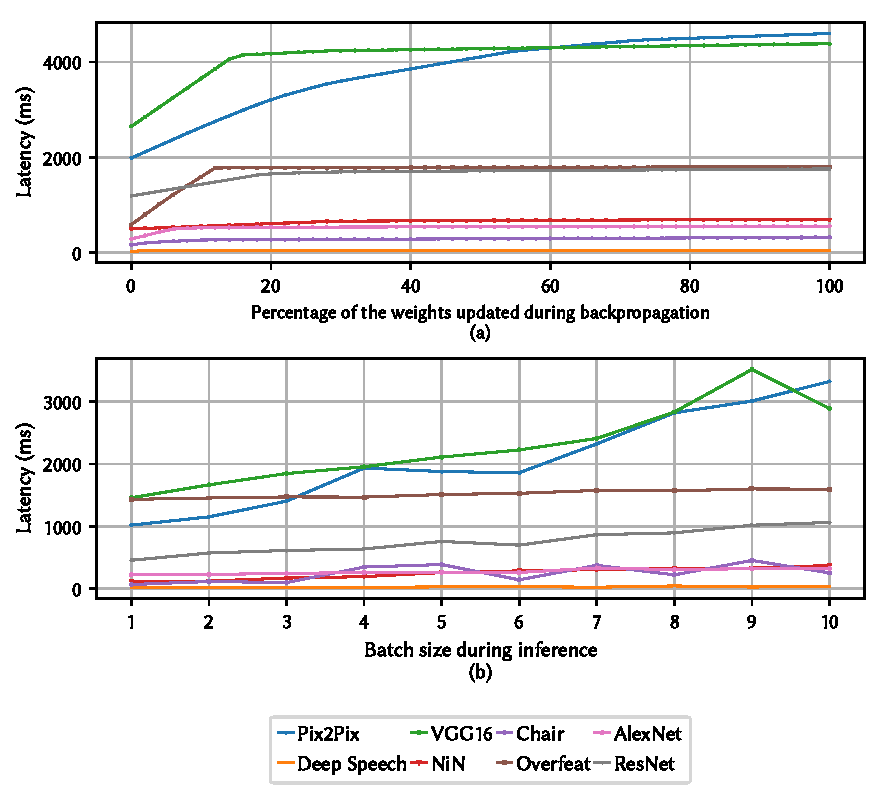
\includegraphics[width=\linewidth]{training_weights_results}
\caption{(a)~Latency of one epoch of online training using JointDNN algorithm vs percentage of updated weights (b)~Latency of mobile-only inference vs. batch size.}\label{weights_changed}
\end{figure}

During online training, the huge communication overhead of transmitting the updated weights will be added to the total cost. Therefore, in order to avoid downloading this large data, only a few back-propagation steps are computed in the cloud server. We performed a simulation by varying the percentage of updated weight. As the percentage of updated weights increases, the latency and energy consumption becomes constant which is shown in~Figure~\ref{weights_changed}. This is the  result of the fact that all the back-propagations will be performed on the mobile device and weights are not transfered from the cloud to the mobile. JointDNN can achieve improvements up to 73\% in latency and 56\% in energy consumption during inference.

\begin{figure}[t]
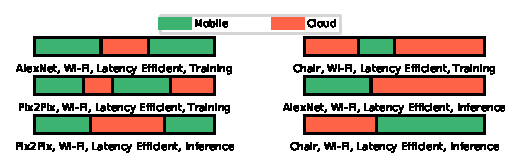
\includegraphics{interesting_patterns}
\caption{Interesting schedules of execution for three types of DNN architectures.} \label{interesting_patterns}
\end{figure}

Different patterns of scheduling are demonstrated in Figure~\ref{interesting_patterns}. They represent the optimal solution in Wi-Fi network while optimizing for latency. They show how the computations in DNN is divided between the mobile and the cloud. As it can be seen, discriminative models (e.g. AlexNet), inference follows a mobile-cloud pattern and training follows a mobile-cloud-mobile pattern. The intuition is that the last layers are computationally intensive \textit{(fc)} with small data sizes, which require a low communication cost, therefore, last layers tend to be computed on the cloud. For generative models (e.g. Chair), the execution schedule of inference is the opposite of discriminative networks, in which the last layers are generally huge and in the optimal solution they are computed on the mobile. Lastly, for autoencoders, where both the input and output data sizes are large, the first and last layers are computed on the mobile.

% \begin{figure}
% 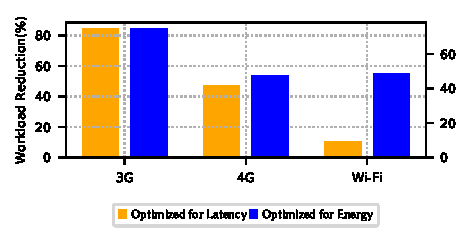
\includegraphics{cloud_improvement}
% \caption{Workload reduction of the cloud server in different mobile networks} \label{cloud_improvement}
% \end{figure}

JointDNN pushes some parts of the computations toward the mobile device. As a result this will lead to less workload on the cloud server. As we see in Table~\ref{cloud_improvement}, we can reduce the cloud server's workload up to 84\% and 53\% on average, which enables the cloud provider to service more users, while obtaining higher performance and lower energy consumptions compared to single-platform approaches.  

\begin{table}[h]
\centering
\caption{Workload reduction of the cloud server in different mobile networks}
\label{cloud_improvement}
\begin{tabular}{|c|c|c|c|}
\hline
\textbf{Optimization Target} & \textbf{3G (\%)} & \textbf{4G (\%)} & \textbf{Wi-Fi (\%)} \\ \hline
Latency                      & 84               & 49               & 12                  \\ \hline
Energy                       & 73               & 49               & 51                  \\ \hline
\end{tabular}
\end{table}

\subsection{Communication Dominance}
Execution time and energy breakdown for AlexNet, which is noted as a representative for the state-of-the-art architectures deployed in cloud servers, is depicted in Figure~\ref{alexnet_extracted}. The cloud-only approach is dominated by the communication costs. As demonstrated in Figure~\ref{alexnet_extracted}, 99\%, 93\% and 81\% of the total execution time is used for communication in case of 3G, 4G, and Wi-Fi, respectively. This relative portion also applies to energy consumption. Comparing the latency and energy of the communication to those of mobile-only approach, we notice that mobile-only approach for AlexNet is better than the cloud-only approach in all the mobile networks. We apply lossless compression methods in order to reduce the effect of the communication, which will be covered in the next section. 

\begin{figure}[t]
\centering
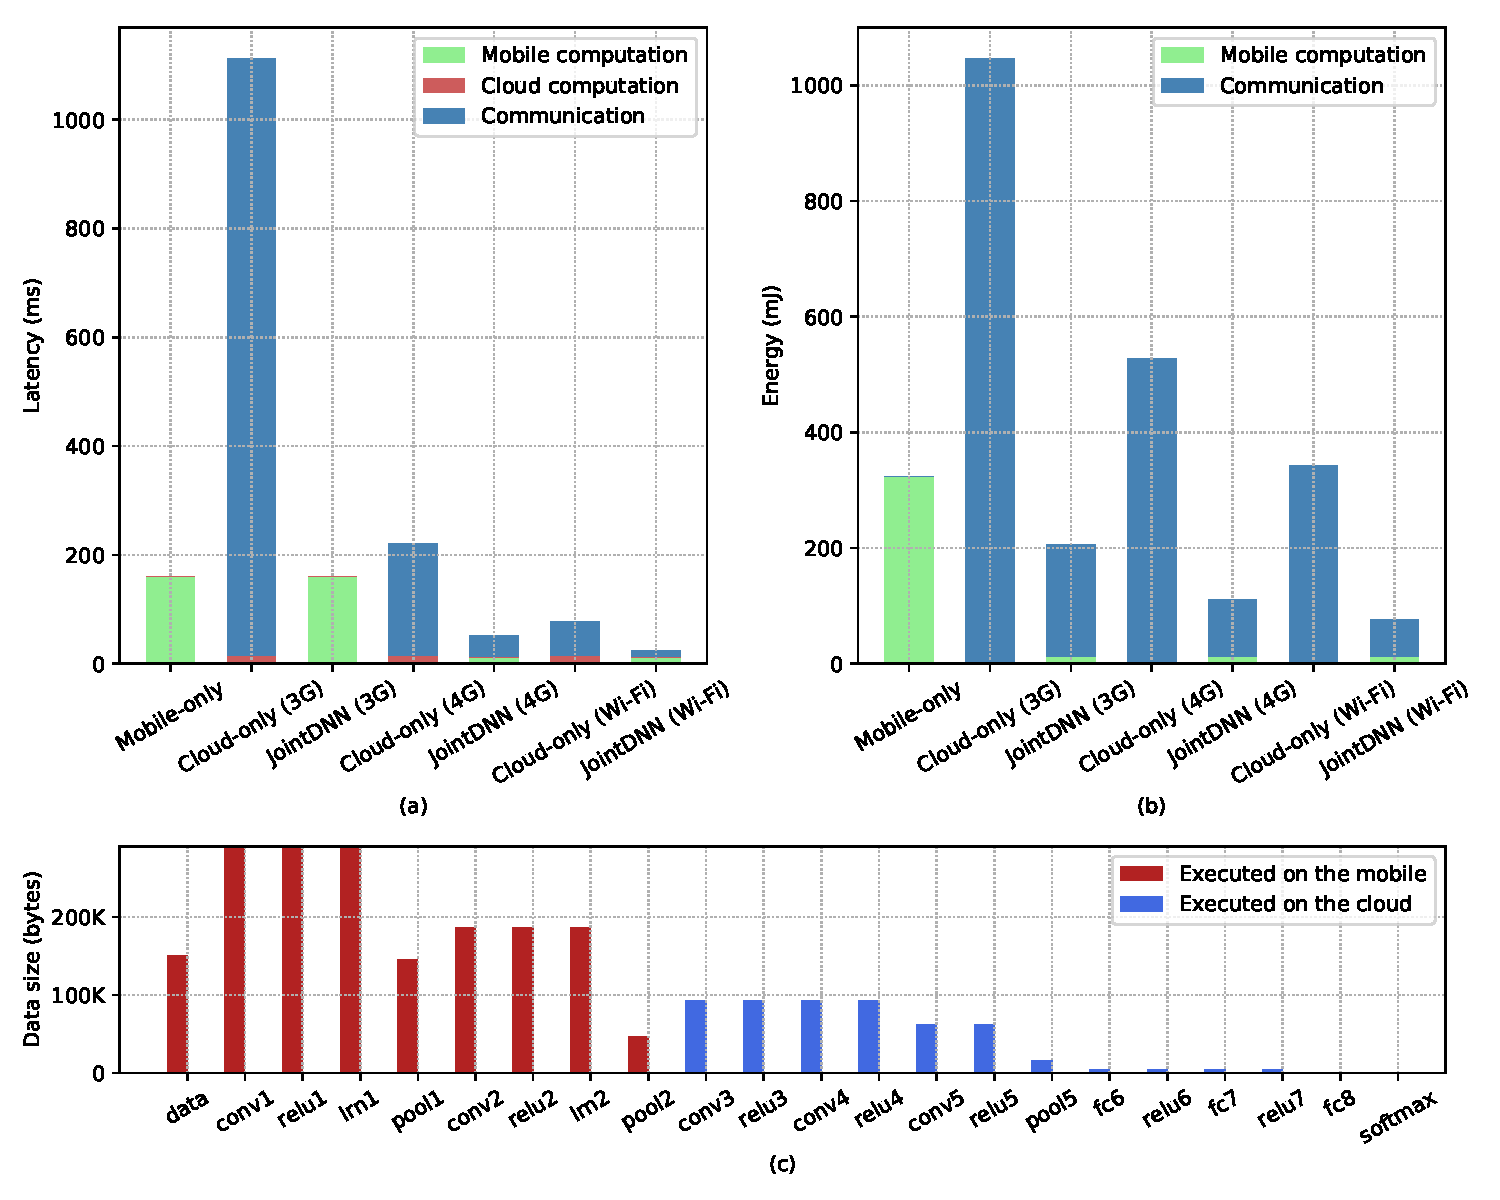
\includegraphics[width=\linewidth]{alexnet_extracted}
\caption{(a) Execution time of AlexNet optimized for performance (b) Mobile energy consumption of AlexNet optimized for energy (c) Data size of the layers in AlexNet and the scheduled computation, where the first nine layers are computed on the mobile and the rest on the cloud, which is the optimal solution w.r.t. both performance and energy.}
\label{alexnet_extracted}
\end{figure}


\subsection{Layer Compression}

The preliminary results of our experiments show that more than $75\%$ of the total energy and delay cost in DNNs are caused by communication in the collaborative approach. This cost is directly proportional to the size of the layer being downloaded to or uploaded from the mobile device. Because of the complex feature extraction process of DNNs, the size of some of the intermediate layers are even larger than network's input data. For example, this ratio can go as high as $10\times$ in VGG16. To address this bottleneck, we investigated compression of the data before any communication. This process can be applied to different DNN architecture types; however, we only considered CNNs due to their specific characteristics explained later in details. 

\begin{figure}[b]
\centering
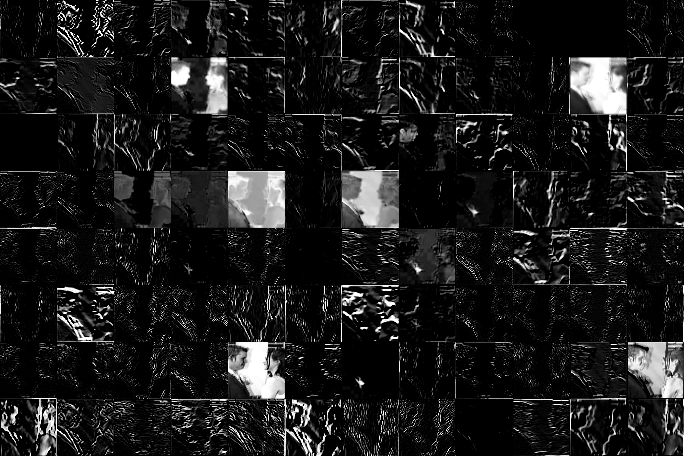
\includegraphics[width=\linewidth]{picCNN}
\caption{Layer output after passing the input image through \textit{conv}, \textit{relu} and \textit{lrn}. Channels are preserving the general structure of the input image and large ratio of the output data is black (zero) due to existence of \textit{relu}. Tiling is used to put all 96 channels together.}
\label{fig:picCNN}
\end{figure}

CNN architectures are mostly used for image and video recognition applications. Because of the spatially local preservation characteristics of \textit{conv} layers, we can assume that the output of the first convolution layers are following the same structure as the input image, as shown in Figure~\ref{fig:picCNN}. Moreover, a big ratio of layer outputs are expected to be zero due to the presence of the relu layer. Our observations shows that the ratio of neurons equal to zero \textit{(ZR)} varies from 50\% to 90\% after \textit{relu} in CNNs. These two characteristics, layers being similar to the input image, and large proportion of their data being a single value, suggest that we can employ existing image compression techniques to their output. 


% This can be ignored! Specially if we don't want to bring that one PNG and JPEG sentence! 
There are two general categories of compression techniques, lossy and lossless~\cite{InformationTheoryCover}. In lossless techniques it is possible to reconstruct the original information completely. On the contrary, lossless techniques use approximations and the original data cannot be reconstructed. In our experiments, we examined the impact of compression using PNG, a lossless technique, based on encoding of frequent sequences in an image. 

% Quantization %% UP TO HERE!
Even though the data type of DNN parameters in typical implementations are 32-bits floating-points, most image formats are based on 3-bytes RGB color triples. Therefore, to compress the layer in the same way as 2D pictures, the floating-point data should be quantized into 8-bits fixed-point. Recent studies show representing the parameters of DNNs with only 4-bits affect the accuracy not more than 1\%~\cite{efficientDNN}. In this work, we implemented our architectures with 8-bits fixed-point and presented our baseline without any compression. 
% Quantization can be applied simply by linear mapping considering uniform distance between each quantization level and converted the 32-bits floating-points into 8-bits. 
% Lossless compression PNG
The layers of CNN contain numerous channels of 2D matrices, each similar to an image. A simple method is to compress each channel separately. In addition to extra overhead of file header for each channel, this method will not take the best of the frequent sequence decoding of PNG. One alternative is locating different channels side by side, referred to as tiling, to form a large 2D matrix representing one layer as shown in Figure~\ref{fig:picCNN}. It should be noted that 1D \textit{fc} layers are very small and we did not apply compression on them.

The Compression Ratio \textit{(CR)} is defined as the ratio of the size of the layer (8-bit) to the size of the compressed 2D matrix in PNG. Looking at the results of compression for two different CNN architectures in Figure~\ref{fig:picCR_VGG}, we can observe a high correlation between ratio of pixels being zero \textit{(ZR)} and \textit{CR}. PNG can compress the layer data up to $5.8\times$ and $3.5\times$ by average. These results confirm the effectiveness of the proposed compression method. By replacing the compressed layers output and adding the cost of compression process itself in JointDNN formulations, we achieve an extra $4.9\times$ and $4.6\times$ improvements in energy and latency on average, respectively.

\begin{figure}[h]
\centering
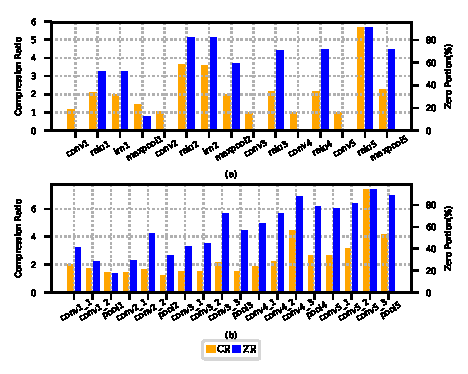
\includegraphics[width=\linewidth]{alexnet_vgg_compression}
\caption{Compression Ratio (CR) and ratio of zero valued neurons (ZR) for different layers of (a) AlexNet and (b) VGG16.}
\label{fig:picCR_VGG}
\end{figure}




\section{Related work and comparison}

\textbf{General Task Offloading Frameworks.} There are existing prior arts focusing on offloading computation from the mobile to the cloud\cite{Oedessa, Comet, CloneCloud, MAUI, ExecutionJavaScript, Refactoring}. However, all these frameworks share a limiting feature that makes them impractical for computation partitioning of the DNN applications. 


These frameworks are programmer annotations dependent as they make decisions about pre-specified functions, whereas JointDNN makes scheduling decisions based on the model topology and mobile network specifications in run-time. Offloading in function level, cannot lead to efficient partition decisions due to layers of a given type within one architecture can have significantly different computation and data characteristics. For instance, a specific convolution layer structure can be computed on mobile or cloud in different models in the optimal solution. 

Neurosurgeon is the only prior art exploring a similar computation offloading idea in DNNs between the mobile device and the cloud server at layer granularity. Neurosurgeon assumes that there is only one data transfer point and the execution schedule of the efficient solution starts with mobile and then switches to the cloud, which performs the whole rest of the computations. Our results show this is not true especially for online training, where the optimal schedule of execution often follows the mobile-cloud-mobile pattern. Moreover, generative and autoencoder models follow a multi data transfer points pattern. Also, the execution schedule can start with the cloud especially in case of generative models where the input data size is large. Furthermore, inter-layer optimizations performed by DNN libraries are not considered in Neurosurgeon. Moreover, Neurosurgeon only schedules for optimal latency and energy, while JointDNN adapts to different scenarios including battery limitation, cloud server congestion, and QoS. Lastly, Neurosurgeon only targets simple CNN and ANN models, while JointDNN utilizes a graph based approach to handle more complex DNN architectures like ResNet and RNNs.
\section{Conclusions}
In this paper, we demonstrated that the status-quo approaches, cloud-only or mobile-only, are not optimal with regard to latency and energy. We reduced the problem of partitioning the computations in a DNN to shortest path problem in a graph. Adding constraints to the shortest path problem makes it NP-Complete, therefore, we also provided ILP formulations to cover different possible scenarios of limitations of mobile battery, cloud congestion, and QoS. One can solve this problem for different set of parameters beforehand (e.g. network bandwidth, cloud server load, etc.) and use a look-up table accordingly to avoid the overhead of solving the optimization problem. The output data size in discriminative networks is typically smaller than other layers in the network, therefore, last layers are expected to be computed on the cloud, while first layers are expected to be computed on the mobile. A reverse reasoning works for Generative models. Autoencoders have large input and output data sizes, which implies that the first and last layers are expected to be computed on the mobile. With these insights, the execution schedule of DNNs can possibly have various patterns depending on the model architecture.




\begin{acks}
This research was supported by grants from NSF SHF and DARPA MTO. 
\end{acks}

\bibliographystyle{ACM-Reference-Format}
\bibliography{sample-bibliography}

\end{document}
